
\subsection{Semantic Segmentation}
We trained our semantic segmentation model on all available datasets, including LAC, Open3D, and LuSNAR. The model was trained to predict seven semantic classes: fiducial markers, rocks, lander, regolith, sky, mountains, and craters. Note that not all datasets contain all classes - for instance, the LAC dataset does not include craters or mountains. Here, we present the results specifically for the LuSNAR dataset, which does not contain landers or fiducial markers. The training was conducted on approximately 8,000 images, with 1,000 images used for validation and 2,000 images from different scenes reserved for testing. The model was trained for 10 epochs using the Adam optimizer with an initial learning rate of $1\times10^{-3}$. We implemented a learning rate schedule with a reduction factor of 0.75, patience of 10 epochs, and a minimum learning rate of $1\times10^{-7}$. The batch size was set to 24 images.

Figure \ref{fig:lusnar_losses} shows the training losses for the different models, showing good convergence. Figure \ref{fig:lusnar_predictions} shows the predictions of different models on the test set, which are able to successfully segment the craters, rocks, regolith, and sky. \Cref{tab:semantic_segmentation_models} shows the quantitative results for the different models on the LuSNAR dataset. We see that FPN performs best in crater detection, U-Net++ in rock detection, and LinkNet shows good overall. PSPNet is outperfoms the rest in terms of computational cost, measured in frames per second (FPS), which is highly desirable for aerospace applications where computational resources are limited. We found the U-Net++ performed well on the Open3D and LAC datasets, and was our choice perform the initial 3D reconstruction experiments.

\begin{figure*}[h]
	\centering
	\begin{subfigure}[b]{0.48\linewidth}
		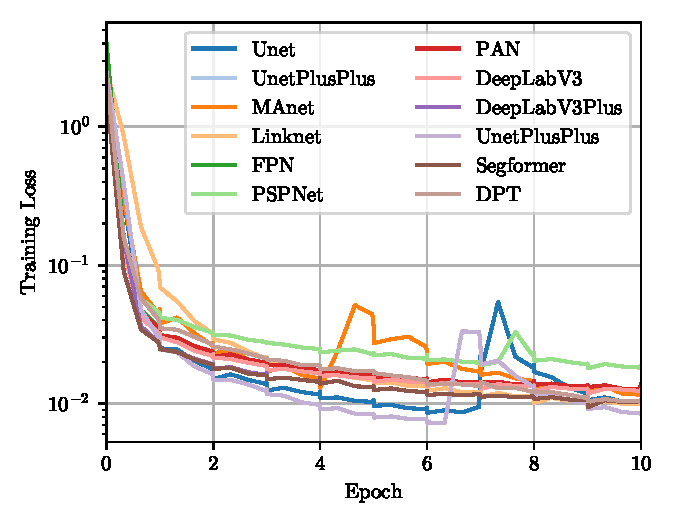
\includegraphics[width=\linewidth]{seg_2d/figures/LuSNAR_losses.pdf}
		\caption{\bfseries Training losses.}
		\label{fig:lusnar_losses}
	\end{subfigure}
	\hfill
	\begin{subfigure}[b]{0.48\linewidth}
		\includegraphics[width=\linewidth]{seg_2d/figures/LuSNAR_losses_val.pdf}
		\caption{\bfseries Validation losses.}
		\label{fig:lusnar_val_losses}
	\end{subfigure}
	\caption{\bfseries Training and validation losses.}
\end{figure*}
% \begin{figure}[h]
%     \centering
%     \begin{subfigure}[b]{\linewidth}
%         \centering
%         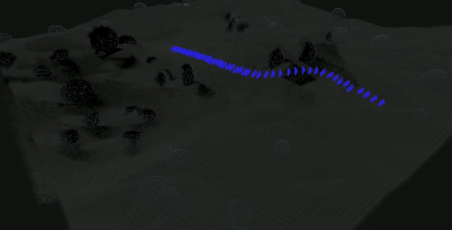
\includegraphics[width=0.8\textwidth]{gaussians_1.png}
%         \caption{\bfseries Ground truth depth and segmentation.}
%         \label{fig:gaussians_1}
%     \end{subfigure}
%     \begin{subfigure}[b]{\linewidth}
%         \centering
%         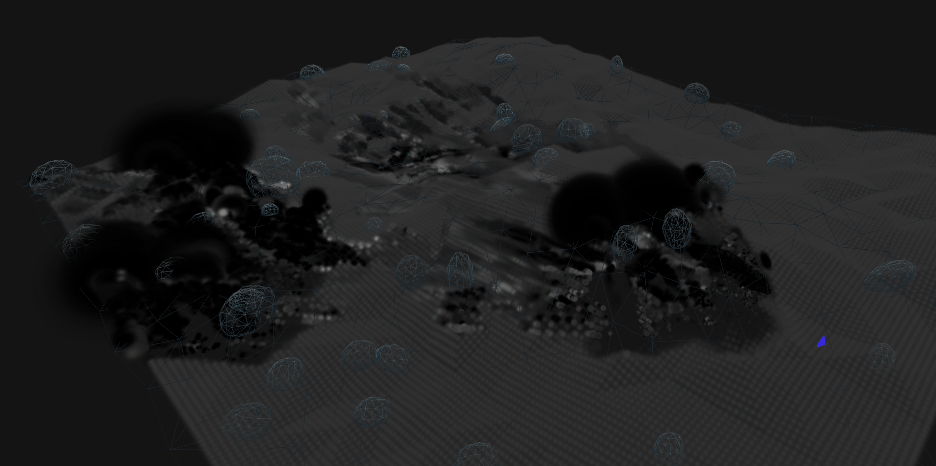
\includegraphics[width=0.8\textwidth]{gaussians_3.png}
%         \caption{\bfseries RAFT-Stereo depth and U-Net++ segmentation.}
%         \label{fig:gaussians_3}
%     \end{subfigure}
%     \caption{\bfseries Effect of depth estimation and segmentation on 3D Gaussian Splatting.}
% \end{figure}


\begin{figure}[t]
	\centering
	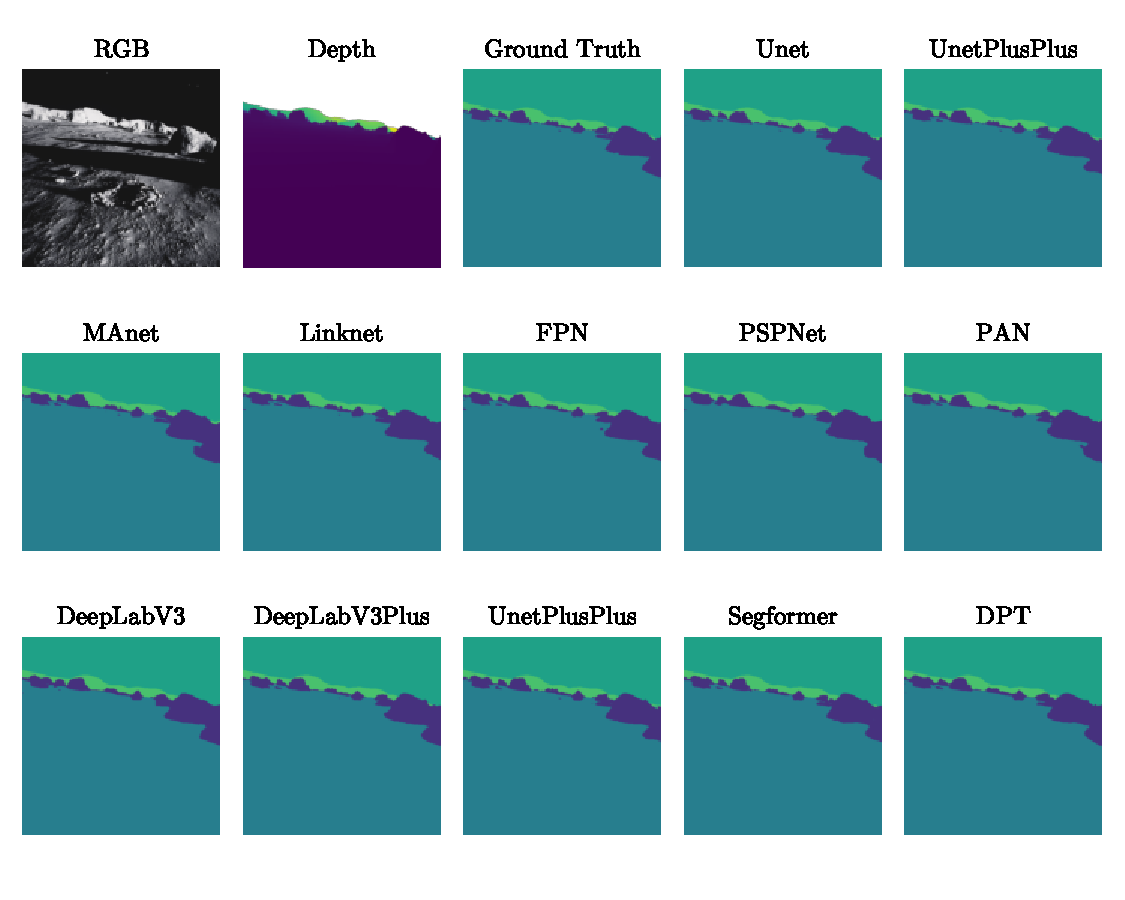
\includegraphics[width=\linewidth, trim={0 0em 0 0em}, clip]{seg_2d/figures/LuSNAR_predictions.pdf}
	\caption{\bfseries Predictions.}
	\label{fig:lusnar_predictions}
\end{figure}

\begin{table*}[h]
	\centering
	\caption{\bfseries Semantic segmentation results on the LuSNAR dataset.}
	\label{tab:semantic_segmentation_models}
	\small
	\begin{tabular}{|l rrrrrrrrrr|}
		\hline
		\multicolumn{1}{|c}{\multirow{2}{*}{\textbf{Model}}}         &
		\multicolumn{1}{c}{\multirow{2}{*}{\textbf{Size [MB]}}}      &
		\multicolumn{1}{c}{\multirow{2}{*}{\textbf{Params}}}         &
		\multicolumn{1}{c}{\multirow{2}{*}{\textbf{FPS $\uparrow$}}} &
		\multicolumn{5}{c}{\textbf{IoU [\%] $\uparrow$}}             &
		\multicolumn{1}{c}{\textbf{Mean}}                            &
		\multicolumn{1}{c|}{\textbf{Mean}}
		\\
		\cmidrule{4-7}
		                                                             &              &               &                &
		\textbf{Regolith}                                            &
		\textbf{Crater}                                              &
		\textbf{Rock}                                                &
		\textbf{Mountain}                                            &
		\textbf{Sky}                                                 &
		\multicolumn{1}{c}{\textbf{IoU $\uparrow$}}                  &
		\multicolumn{1}{c|}{\textbf{Accuracy $\uparrow$}}
		\\
		\hline
		\hline
		U-Net                                                        & 55.0         & 14.3M         & 114.4          & \textbf{99.5} & 95.5          & 89.2          & 96.5          & \textbf{99.8} & 96.1          & 99.5          \\
		U-Net++                                                      & 61.0         & 16.0M         & 78.0           & \textbf{99.5} & 91.1          & \textbf{91.6} & \textbf{98.5} & \textbf{99.8} & 96.1          & \textbf{99.6} \\
		MA-Net                                                       & 83.0         & 21.7M         & 71.7           & 99.2          & 70.9          & 90.1          & 97.5          & \textbf{99.8} & 91.5          & 99.3          \\
		Linknet                                                      & 44.0         & 11.7M         & 104.5          & 99.2          & 96.4          & 91.1          & 97.0          & \textbf{99.8} & \textbf{96.7} & 99.3          \\
		FPN                                                          & 50.0         & 13.0M         & 108.7          & 98.9          & \textbf{97.7} & 86.8          & 97.8          & 99.7          & 96.2          & 99.2          \\
		PSPNet                                                       & \textbf{3.0} & \textbf{0.9M} & \textbf{203.2} & 98.8          & 92.7          & 79.7          & 94.3          & 99.6          & 93.0          & 99.0          \\
		PAN                                                          & 43.0         & 11.4M         & 92.8           & 99.0          & 94.6          & 84.3          & 97.4          & 99.7          & 95.0          & 99.2          \\
		DeepLabV3                                                    & 61.0         & 15.9M         & 131.5          & 99.0          & 96.7          & 86.6          & 98.3          & 99.7          & 96.1          & 99.2          \\
		DeepLabV3Plus                                                & 47.0         & 12.3M         & 118.8          & 99.2          & 96.4          & 89.2          & 98.0          & \textbf{99.8} & 96.5          & 99.4          \\
		Segformer                                                    & 45.0         & 11.8M         & 140.5          & 99.2          & 95.5          & 88.9          & 97.7          & \textbf{99.8} & 96.2          & 99.4          \\
		DPT                                                          & 159.0        & 41.6M         & 79.6           & 99.1          & 94.1          & 87.4          & 95.7          & 99.7          & 95.2          & 99.3          \\
		\hline
	\end{tabular}
\end{table*}